% !TEX root = main.tex
\chapter{Das Standardmodell der Teilchenphysik}

Im folgenden Kapitel werden die grundlegenden Teilchen und Wechselwirkungen des Standard Modells der Teilchenphysik beschrieben. In Anlehnung an \cite{Perkins:396126,Peskin:257493} folgt dazu zunächst ein kurzer Überblick über alle fundamentalen Teilchen. Daran anschließend werden die dem Modell zugrunde liegenden diskreten Symmetrien erläutert. Abschließend wird zunächst der Mechanismus, in dem neutrale $\B$-Mesonen mischen, beschrieben, um dann auf die $\CP$-Verletzung einzugehen , für deren Messung das Flavour Tagging bei \lhcb eine Grundlage bildet (Erläuterungen auf Basis von \cite{Bigi:1295518,Branco:396964}). 

\section{Grundlagen}\label{sec:grundlagen}

Beim Standardmodell (SM) der Teilchenphysik handelt es sich um eine relativistische Quantenfeldtheorie. Teilchen werden durch Felder $\phi(x)$ erzeugt und vernichtet, und die Dynamik wird wie in der klassischen Physik durch die Lagrangefunktion $\mathcal{L}(\phi(x),\partial_\mu\phi(x))$ beschrieben. Insgesamt gibt es zwölf fundamentale Teilchen mit halbzahligem Spin, sechs Quarks und sechs Leptonen. Diese Teilchen werden Fermionen genannt, im Gegensatz zu Teilchen mit ganzzahligem Spin, den sogenannten Bosonen. Die Fermionen bilden jegliche Materie, während die Bosonen als Austauschteilchen der Kräfte im SM fungieren (Abbildung \ref{fig:SM_teilchen}).
\begin{figure}[htbp]
	\centering
		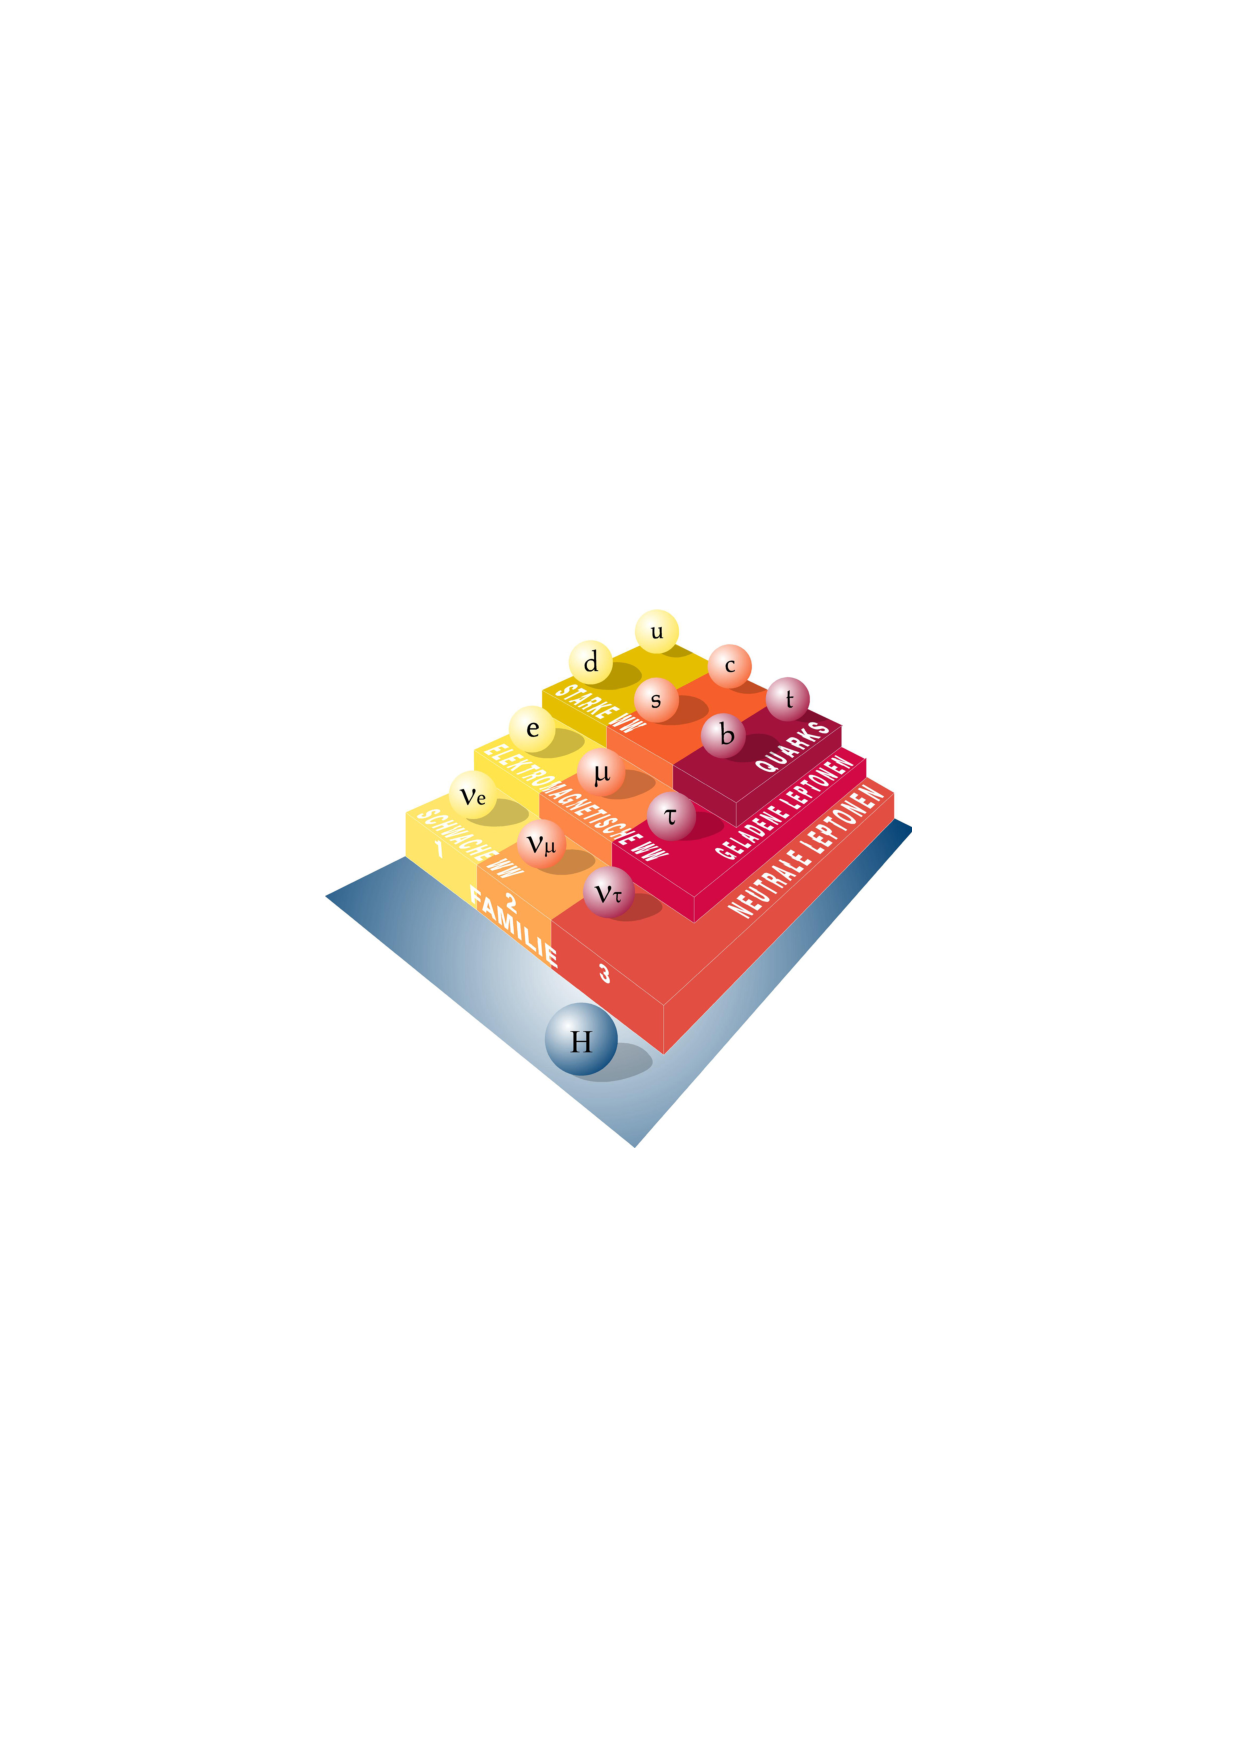
\includegraphics[width=0.5\textwidth]{fig/SM_teilchen.pdf}
	\caption{Fermionen des Standardmodells der Teilchenphysik und auf sie wirkende Kräfte. \cite{SM_teilchen}}
	\label{fig:SM_teilchen} 
\end{figure}\\
Sowohl die Quarks als auch die Leptonen sind in drei Familien unterteilt, wobei jede Familie einem Teilchenduplett entspricht. Bei den Quarks unterscheidet man weiter zwischen Up- und  Down-Type Quarks. Die Up-Type Quarks sind das up- ($\uquark$), charm- ($\cquark$) und top-Quark ($\tquark$), zu den Down-Type-Quarks gehören das down- ($\dquark$), strange- ($\squark$) und bottom-Quark ($\bquark$). Die Up-Type-Quarks tragen eine Ladung von $+\tfrac{2}{3}\electron$, während die Down-Type-Quarks eine Ladung von $-\tfrac{1}{3}\electron$ haben.\\
Bei den Leptonen unterscheidet man zwischen den geladenen Leptonen, dem Elektron ($\en$), dem Myon ($\mun$) und dem Tauon ($\taum$), und den ungeladenen Leptonen, den zugehörigen Neutrinos ($\neue$, $\neum$, $\neut$). Zu jedem dieser zwölf Fermionen gibt es ein zugehöriges Antiteilchen mit umgekehrter Ladung. Bei den Quarks spricht man bei dieser Unterscheidung auch vom sogenannten Flavour.\\
Zu den Bosonen gehören unter anderem die Eichbosonen, die direkt mit den im SM beschriebenen Kräften assoziiert sind. Die acht Gluonen $g$ sind Austauschteilchen der starken Wechselwirkung (WW) und koppeln an die  sogenannte Farbladung. Diese wird von Quarks getragen, die neben ihrer elektrischen Ladung eine Farbladung tragen. Die möglichen Farben sind grün, blau und rot, außerdem gibt es zu jeder Farbe auch eine Antifarbe. Teilchen mit Farbladungen können nicht frei auftreten, sondern müssen immer in gebundenen farbneutralen Zuständen existieren. So treten die Quarks immer in gebunden Zuständen von drei Quarks (Baryonen) mit drei Farben oder drei Antifarben oder in gebundenen Zuständen von zwei Quarks (Mesonen) mit einer Farbe und ihrer Antifarbe auf. Weil von den Fermionen nur die Quarks eine Farbladung tragen, sind diese als einzige Teilchen von der starken WW beeinflusst. Die Gluonen sind masselos und können, da sie eine Farbe und eine Antifarbe tragen, auch an sich selbst koppeln.\\ 
Als zweite WW wird die elektromagnetische WW beschrieben. Diese wird durch das Photon $\g$ vermittelt, das an die elektrische Ladung koppelt , sodass hier die Neutrinos als einzige elementare, ungeladene Fermionen nicht beeinflusst sind. Das Photon ist wie die Gluonen masselos, da es aber auch keine elektrische Ladung trägt, koppelt es nicht an sich selbst.\\ 
Die dritte WW im Standardmodell ist die schwache WW. Ihre Austauschteilchen sind das ungeladene \Z-Boson und die geladenen \Wpm-Bosonen. Im Gegensatz zu den bisher genannten Eichbosonen verfügen diese über Massen von $M_W\approx\SI{80}{GeV}$ und $M_Z\approx\SI{91}{GeV}$ \cite{PDG-2012}. Sie koppeln an alle der zwölf Fermionen.\\ 
Die schwache WW nimmt jedoch noch eine Sonderstellung ein. Sie koppelt an die linkshändigen Dupletts der Quarks und Leptonen. Bei den Leptonen können die Eigenzustände der schwachen WW unter Annahme von masselosen Neutrinos durch eine einfache Transformation in das Eigensystem der Masseneigenzustände der geladenen Leptonen überführt werden. Im Quarksektor ist dies jedoch nicht für beide Quarktypen möglich. Nach Konvention wählt man hier die Up-Type-Quarks, sodass man für die Down-Type-Quarks eine Transformationsmatrix $V_{C\!K\!M}$ zwischen den Eigenzuständen zur schwachen WW $\dquark'$, $\squark'$ und $\bquark'$ und den Masseneigenzuständen $\dquark$, $\squark$ und $\bquark$ erhält:
\begin{equation}
\begin{pmatrix}\dquark'\\ \squark'\\ \bquark'\end{pmatrix}=\begin{pmatrix}\Vud & \Vus & \Vub\\ \Vcd & \Vcs & \Vcb\\ \Vtd & \Vts & \Vtb\end{pmatrix}\begin{pmatrix}\dquark\\ \squark\\ \bquark\end{pmatrix}\approx\begin{pmatrix}1-\frac{\lambda^2}{2} & \lambda & A\lambda^3(\rho-i\eta)\\-\lambda & 1-\frac{\lambda^2}{2} & A\lambda^2\\A\lambda^3(1-\rho-i\eta) & -A\lambda^2 & 1\end{pmatrix}\begin{pmatrix}\dquark\\ \squark\\ \bquark\end{pmatrix}\label{eq:wolfen}
\end{equation}
Diese sogenannte $C\!K\!M$-Matrix hat vier Freiheitsgrade und ist unitär. Sie lässt sich, wie in Gleichung \eqref{eq:wolfen} dargestellt, mit der Wolfenstein Parametrisierung durch drei reelle Parameter ($A$, $\rho$, $\lambda$) und eine komplexe Phase ($\eta$) mit $\lambda\approx0{,}22$ parametrisieren \cite{ckm_param}. Man erkennt, dass die Matrixelemente bei größerer Entfernung von der Diagonalen kleiner werden.\\ 
Als letztes Eichboson gibt es im SM das erst vor kurzem entdeckte Higgs-Boson $\PH$ \cite{higgs_found,higgs_atlas}. Dieses ist Austauschteilchen des Higgs-Feldes und wechselwirkt mit allen massiven Teilchen. Das Higgs-Boson selbst hat eine Masse von $M_H\approx\SI{126}{GeV}$ \cite{PDG-2012}. 

\section{Symmetrien}\label{sec:disksym}

Man unterscheidet im SM zwischen diskreten Symmetrien und kontinuierlichen Eichsymmetrien. Bei den kontinuierlichen Eichsymmetrien wird dabei eine lokale Eichinvarianz gefordert, bei der in den jeweiligen Symmetriegruppen $U(1)$ (elektromagnetische WW), $SU(2)$ (schwache WW) und $SU(3)$ (starke WW) die WW entstehen. Die Eichbosonen treten als Generatoren der jeweiligen Eichtransformationen auf. Dies soll hier für die $U(1)$ Gruppe gezeigt werden. Die Lagrangedichte 
\begin{equation}
\mathcal{L}=\overline{\psi}\left(i\slashed{\partial}-m\right)\psi-\frac{1}{4}F^{\mu\nu}F_{\mu\nu}-\underbrace{eQ\overline{\psi}\gamma^\mu\psi}_{j^\mu} A_\mu
\end{equation}
bleibt  unter den Transformationen
\begin{align}
\psi\rightarrow\psi'&=e^{-ieQ\theta(x)}\psi\\
A_\mu\rightarrow A_\mu'&=A_\mu+\partial_\mu\theta
\end{align}
invariant. Hier lässt sich nun das Eichfeld $A_\mu$ mit dem Photon identifizieren und man erkennt den Wechselwirkungsterm $j^\mu A_\mu$. Fordert man nun für die höheren Symmetriegruppen äquivalent lokale Eichtransformationen, so werden entsprechend die weiteren Eichbosonen erzeugt.\\
Neben diesen kontinuierlichen Symmetrien gibt es außerdem drei diskrete Symmetrien im Standardmodell der Teilchenphysik.
\begin{itemize}
\item Der Paritätsoperator $P$ beschreibt eine Raumspiegelung $P\psi(t,\vec{x})=\psi(t,-\vec{x})$. Der Operator ist unitär, es gilt also $P^\dagger=P^{-1}$.
\item Mit der Ladungskonjugation $C$ wechselt man zwischen einem Teilchen und seinem Antiteilchen. Die Bezeichnung als Ladungskonjugation ist hier etwas irreführend, da auch alle weiteren additiven Quantenzahlen wie die Baryonenzahlen von $C$ beeinflusst werden. Ebenso wie der Paritätsoperator ist auch $C$ unitär.
\item Die dritte diskrete Symmetrie ist die Zeitumkehr $T$. Diese dreht das Vorzeichen der zeitlichen Komponente $T\psi(t,\vec{x})=\psi(-t,\vec{x})$. Im Gegensatz zu den anderen beiden Operatoren ist er jedoch nicht unitär sondern antiunitär, es gilt also $T^2=1$.
\end{itemize}
Die Symmetrien sind sowohl einzeln als auch in Kombination mit jeweils einer weiteren Symmetrie ($P\!T$, $C\!T$, $C\!P$) von der schwachen WW gebrochen. Erst die Kombination \CPT aller drei Symmetrien ist erhalten. Daraus folgen für Teilchen und Antiteilchen gleiche Massen und Lebenszeiten.

\section[head={Mischung von \B-Mesonen},tocentry={Mischung von \B-Mesonen}]{Mischung von $\mathbf{\B}$-Mesonen}\label{sec:mixing}

Wie bereits in Kapitel \ref{sec:grundlagen} erläutert, sind für Quarks Masseneigenzustände und Eigenzustände der schwachen WW, auch Flavoureigenzustände, nicht identisch. Gleiches gilt für aus Quarks zusammengesetzte Teilchen wie $\B$-Mesonen. Betrachtet man nun das Zweiteilchensystem aus \Bz (\bquarkbar\dquark) und \Bzb (\bquark\dquarkbar), so erhält man die zeitliche Entwicklung dieses Systems aus der Schrödingergleichung
\begin{equation}
i\frac{d}{dt}\begin{pmatrix}\Bz\\ \Bzb\end{pmatrix}=\mathcal{H}\begin{pmatrix}\Bz\\ \Bzb\end{pmatrix}=\left(M-\frac{i}{2}\Gamma\right)\begin{pmatrix}\Bz\\ \Bzb\end{pmatrix},
\end{equation}
wobei $M$ und $\Gamma$ hermitesche Matrizen sind. Aufgrund des $\CPT$-Theorems muss außerdem  $m_{11}=m_{22}$ und $\Gamma_{11}=\Gamma_{22}$ gelten. Diagonalisiert man diese Matrix nun erhält man die Eigenwerte $\mu_{1,2}=m_{1,2}-\frac{i}{2}\Gamma_{1,2}$ mit den Massen $m_{1,2}$ und Zerfallsbreiten $\Gamma_{1,2}$ der Masseneigenzustände. Im $\B$-System bezeichnet man  die Masseneigenzustände mit $\B_L$ und $\B_H$ und analog die zugehörigen Massen mit  $m_L$ und $m_H$ sowie die Zerfallsbreiten mit $\Gamma_L$ und $\Gamma_H$. Die Masseneigenzustände ergeben sich dabei zu
\begin{equation}
\begin{split}
\left|B_H\right>&\sim p\left|\Bz\right>-q\left|\Bzb\right>\\
\left|B_L\right>&\sim p\left|\Bz\right>+q\left|\Bzb\right>
\end{split}
\end{equation}
wobei $p$ und $q$ der Normierungsbedingung $\left|p\right|^2+\left|q\right|^2=1$ folgen müssen. Weiterhin lassen sich die Größen 
\begin{align}
\dm&=m_H-m_L\\
\Delta\Gamma&=\Gamma_H-\Gamma_L
\end{align}
definieren, wobei die Massendifferenz $\dm$ als positiv definiert ist. Für die Zeitentwicklung der Flavoureigenzustände erhält man 
\begin{equation}
\begin{split}
\left|\Bz(t)\right>&=\frac{1}{2}\left|\Bz\right>g_+-\frac{q}{2p}\left|\Bzb\right>g_-,\\
\left|\Bzb(t)\right>&=\frac{1}{2}\left|\Bzb\right>g_--\frac{p}{2q}\left|\Bz\right>g_+
\end{split}
\end{equation}
mit $g_\pm=e^{-\mu_Ht}\pm e^{-\mu_Lt}$. Nun lässt sich die Wahrscheinlichkeit berechnen, mit der ein produziertes ($t=0$) $\Bz$-Meson nach einer Zeit $t$ in ein $\Bzb$-Meson oszilliert ist:
\begin{equation}
\left|\left<\Bzb\Big|\Bz(t)\right>\right|^2=\frac{1}{4}\left|\frac{q}{p}\right|^2\left(e^{-\Gamma_Ht}+e^{-\Gamma_Lt}-2e^{\frac{1}{2}\left(\Gamma_H+\Gamma_L\right)t}\cos\left(\dm t\right)\right).\label{eq:uebergang1}
\end{equation}
Man erkennt, dass die Wahrscheinlichkeit eines anfänglichen $\Bz$-Mesons als $\Bzb$-Meson zu zerfallen, mit der Frequenz $\dm$ oszilliert. Ebenso lässt sich die Wahrscheinlichkeit für ein anfängliches $\Bzb$-Meson definieren. Die Feynmangraphen zu beiden Prozessen sind in Abbildung \ref{fig:mixing} zu sehen.\\
Analog zu Gleichung \eqref{eq:uebergang1} lassen sich die Wahrscheinlichkeiten $\left|\left<\Bz\Big|\Bzb(t)\right>\right|^2$, $\left|\left<\Bzb\Big|\Bzb(t)\right>\right|^2$ und $\left|\left<\Bz\Big|\Bz(t)\right>\right|^2$ berechnen:
\begin{align}
\left|\left<\Bz\Big|\Bzb(t)\right>\right|^2&=\frac{1}{4}\left|\frac{p}{q}\right|^2\left(e^{-\Gamma_Ht}+e^{-\Gamma_Lt}-2e^{\frac{1}{2}\left(\Gamma_H+\Gamma_L\right)t}\cos\left(\dm t\right)\right),\label{eq:uebergang2}\\
\left|\left<\Bzb\Big|\Bzb(t)\right>\right|^2&=\frac{1}{4}\left(e^{-\Gamma_Ht}+e^{-\Gamma_Lt}+2e^{\frac{1}{2}\left(\Gamma_H+\Gamma_L\right)t}\cos\left(\dm t\right)\right),\label{eq:uebergang3}\\
\left|\left<\Bz\Big|\Bz(t)\right>\right|^2&=\frac{1}{4}\left(e^{-\Gamma_Ht}+e^{-\Gamma_Lt}+2e^{\frac{1}{2}\left(\Gamma_H+\Gamma_L\right)t}\cos\left(\dm t\right)\right).\label{eq:uebergang4}
\end{align}
Ohne $\CP$-Verletzung in der Mischung (siehe Abschnitt \ref{sec:cpv}) lässt sich eine Mischungsasymmetrie berechnen:
\begin{equation}
\begin{split}
A_{\text{mix}}(t)&=\frac{\left(\Gamma(\Bz(t)\rightarrow\Bz)+\Gamma(\Bzb(t)\rightarrow\Bzb)\right)-\left(\Gamma(\Bzb(t)\rightarrow\Bz)+\Gamma(\Bz(t)\rightarrow\Bzb)\right)}{\left(\Gamma(\Bz(t)\rightarrow\Bz)+\Gamma(\Bzb(t)\rightarrow\Bzb)\right)+\left(\Gamma(\Bzb(t)\rightarrow\Bz)+\Gamma(\Bz(t)\rightarrow\Bzb)\right)}\\
&=\frac{N_\text{unmixed}(t)-N_\text{mixed}(t)}{N_\text{unmixed}(t)+N_\text{mixed}(t)}=\cos(\dm t).\label{eq:mixing}
\end{split}
\end{equation}
Dabei ist $N_\text{unmixed}(t)$ die Anzahl der nicht oszillierten $\B$-Mesonen und $N_\text{mixed}(t)$ die Anzahl der oszillierten $\B$-Mesonen zum Zeitpunkt $t$. Für  \Bz-Mesonen gilt außerdem $\Gamma_H\approx\Gamma_L$.
\begin{figure}[htbp]
	\begin{center}
		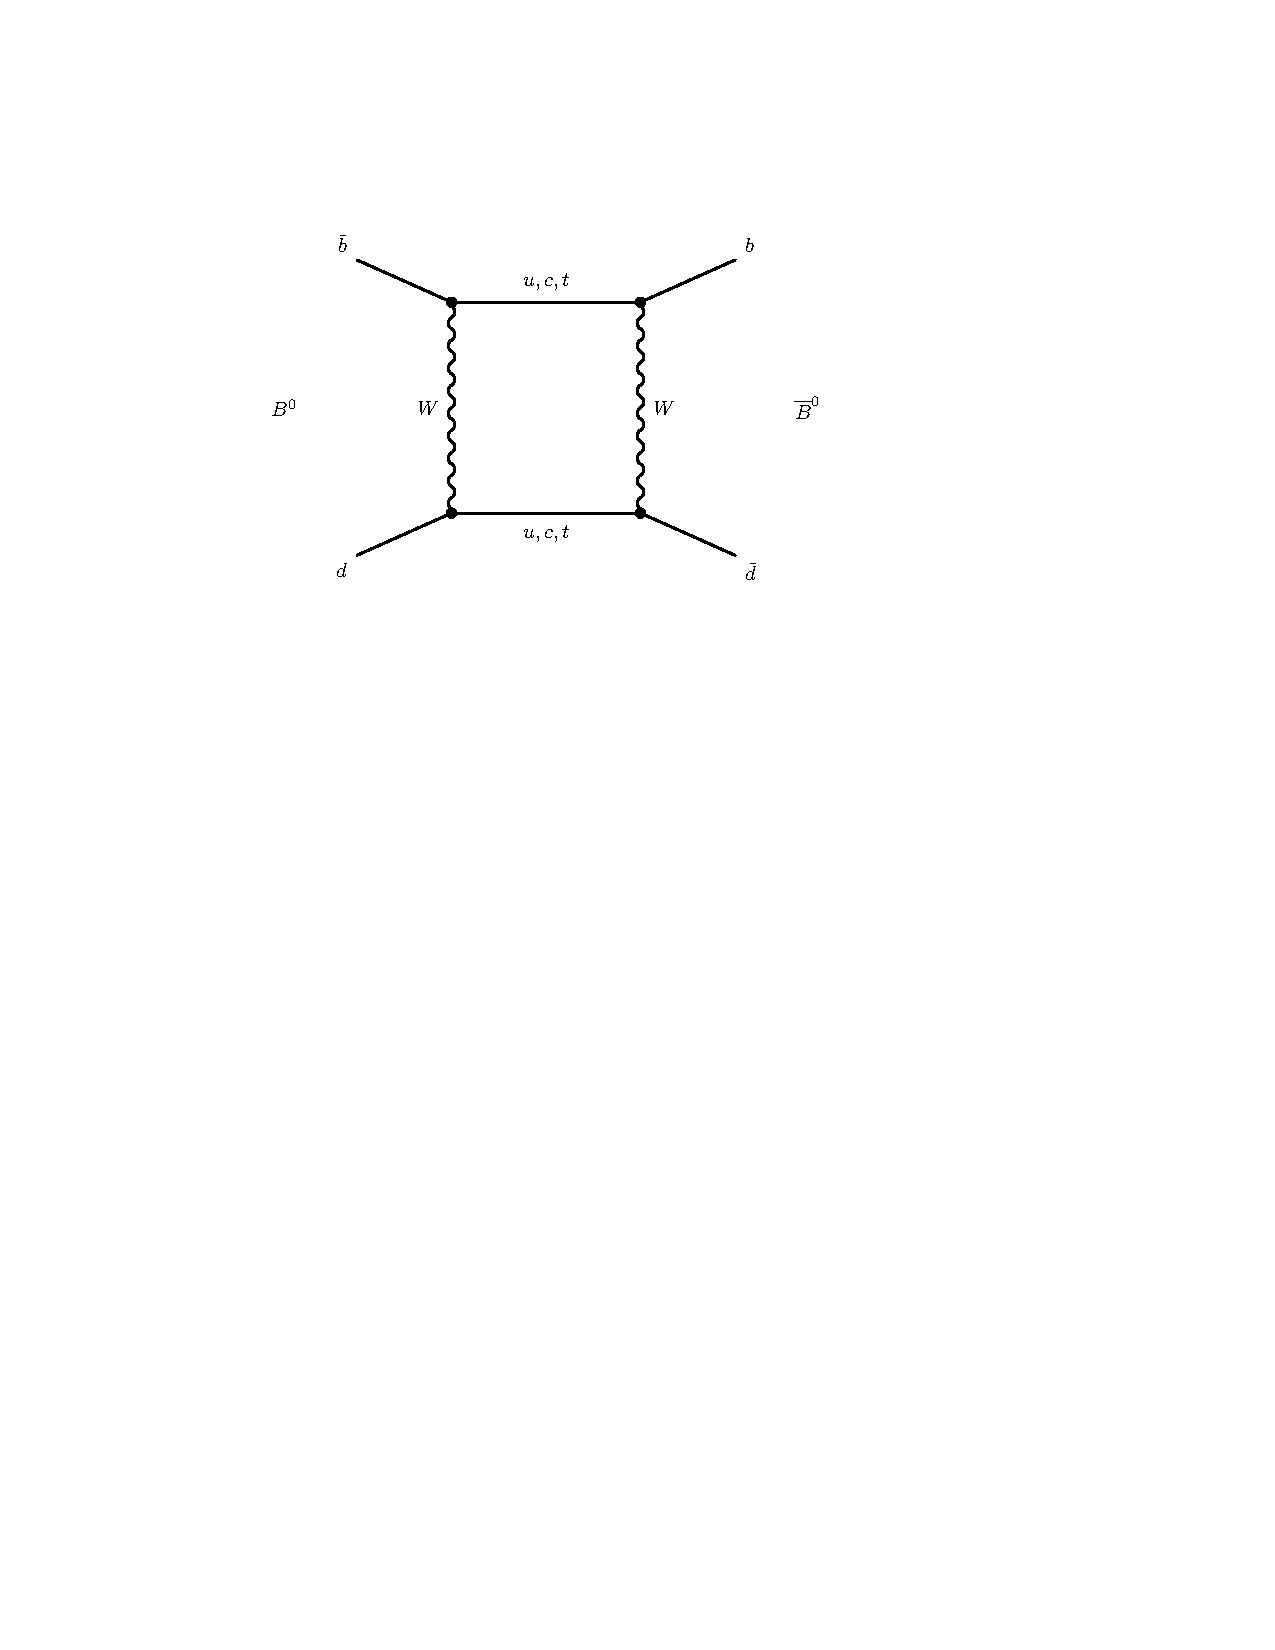
\includegraphics[width=0.45\textwidth]{fig/B_mixing_1.pdf}
		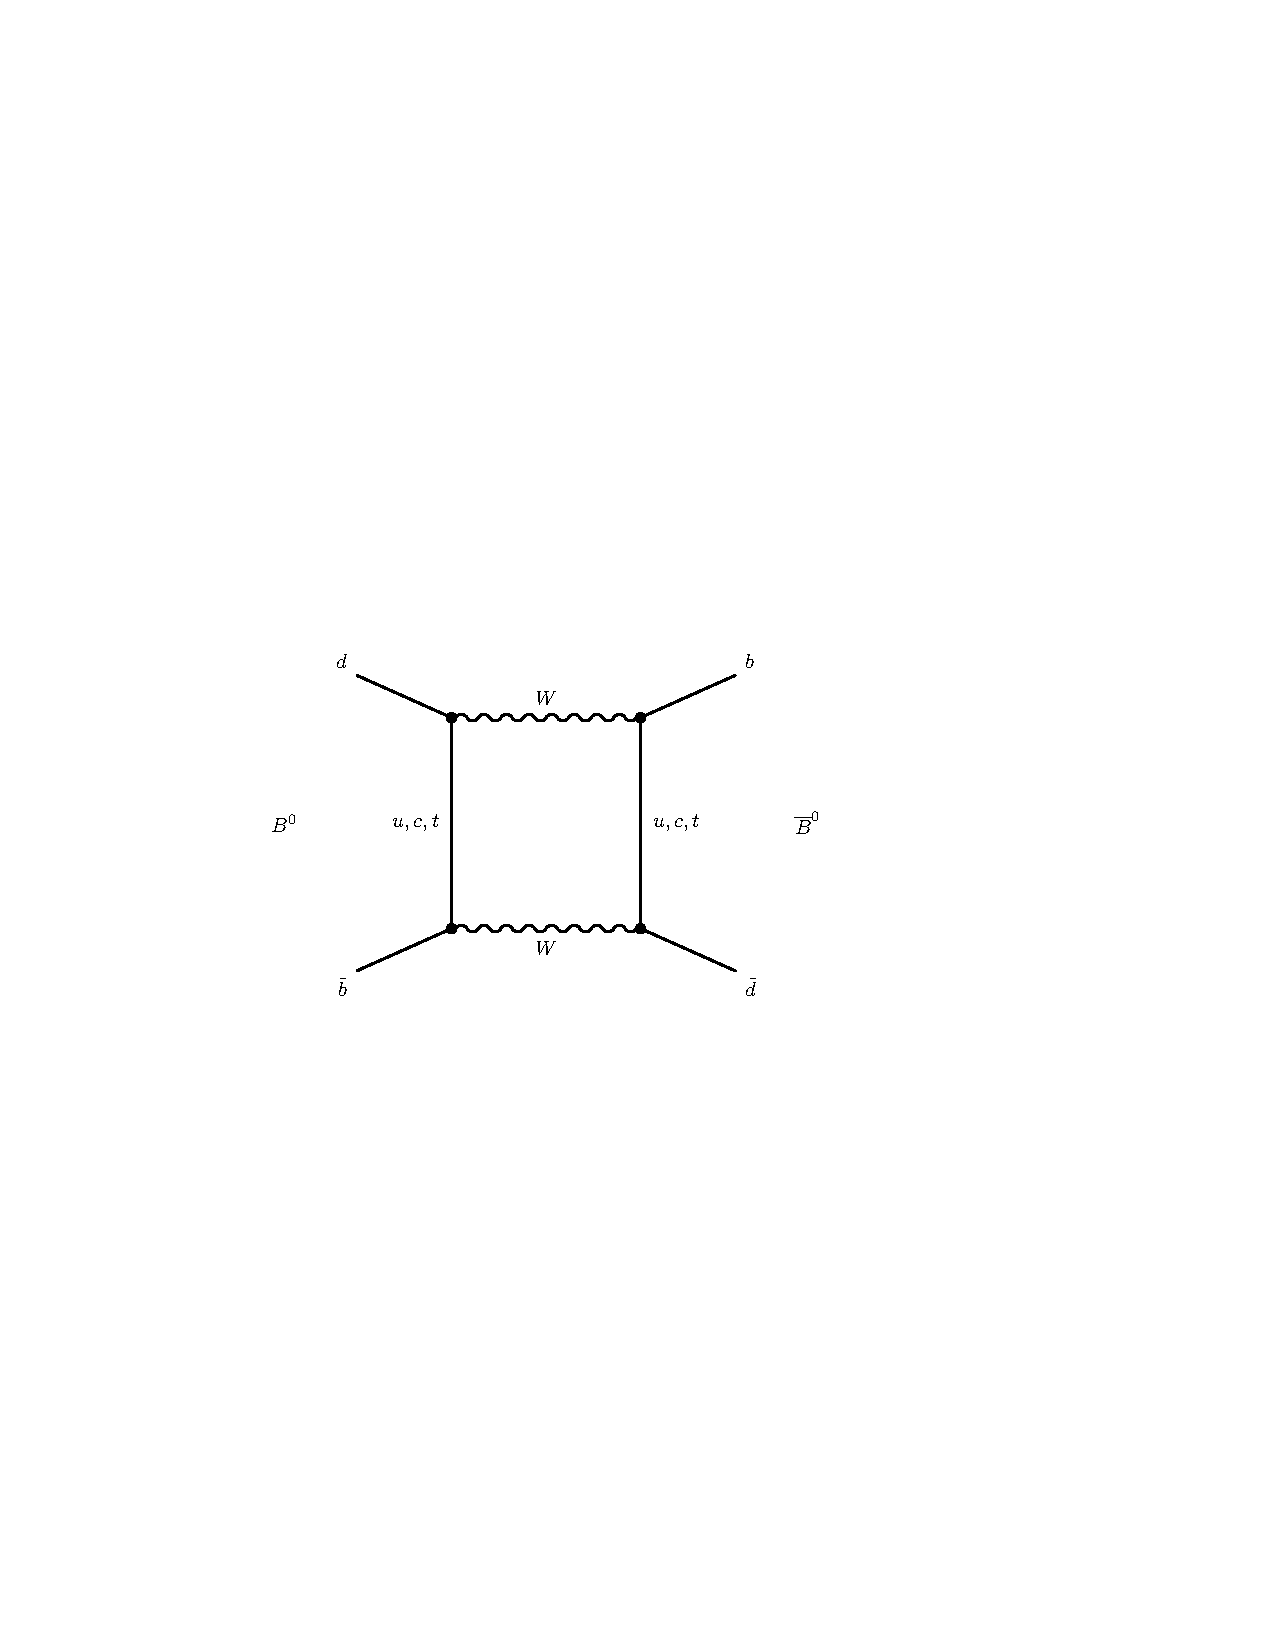
\includegraphics[width=0.45\textwidth]{fig/B_mixing_2.pdf}
	\caption{Box-Diagramme niedrigster Ordnung zur Oszillation neutraler \Bz-Mesonen. Dominiert werden beide Diagramme vom $\tquark$-Quark.}
	\label{fig:mixing}
 	\end{center}
\end{figure}

\section[head={$\CP$-Verletzung},tocentry={$\CP$-Verletzung}]{$\mathbf{CP}$-Verletzung}\label{sec:cpv}

Die $\CP$-Symmetrie ist, wie in Kapitel \ref{sec:disksym} angemerkt, von der schwachen WW gebrochen. Um zwischen den verschiedenen Arten der $\CP$-Verletzung zu unterscheiden, sollen zunächst vier Zerfallsamplituden eingeführt werden
\begin{equation}
\begin{split}
A_f=\left<f\big|T\big|\Bz\right>&\hspace{1.5cm}\overline{A}_f=\left<f\Big|T\Big|\Bzb\right>\\
A_{\bar{f}}=\left<\bar{f}\Big|T\Big|\Bz\right>&\hspace{1.5cm}\overline{A}_{\bar{f}}=\left<\bar{f}\Big|T\Big|\Bzb\right>,
\end{split}
\end{equation}
wobei $T$ die Übergangsmatrix zwischen dem $\B$-Meson und einem beliebigen Endzustand $f$ darstellt. Nun lässt sich zwischen drei Arten von $\CP$-Verletzung unterscheiden:
\begin{itemize}
\item Direkte $\CP$-Verletzung, oder auch $\CP$-Verletzung im Zerfall, bedeutet, dass sich die Zerfallsamplituden zwischen $\Bz$ und $\Bzb$-Meson unterscheiden. Es gilt also $\left|A_f\right|\neq\left|\overline{A}_{\bar{f}}\right|$ und $\left|A_{\bar{f}}\right|\neq\left|\overline{A}_f\right|$
\item Bei der indirekten $\CP$-Verletzung ($\CP$-Verletzung in der Mischung) sind die Übergangswahrscheinlichkeiten von $\Bz$ nach $\Bzb$ und andersherum voneinander verschieden. Für die Matrixelemente bedeutet dies, dass $\left|\left<\Bzb\Big|\Bz(t)\right>\right|\neq\left|\left<\Bz\Big|\Bzb(t)\right>\right|$ und damit $\left|\tfrac{q}{p}\right|\neq1$. 
\item Die dritte Art der $\CP$-Verletzung kann in der Interferenz von Mischung und Zerfall auftreten. Im einfachsten Fall zerfallen beide Flavoureigenzustände in einen gemeinsamen Endzustand. Allgemein gilt für diese Art der $\CP$-Verletzung $\left<f\big|T\big|\Bz(t)\right>\neq\left<\bar{f}\Big|T\Big|\Bzb(t)\right>$. Betrachtet man nun die Größe
\begin{equation}
\lambda_f=\frac{q}{p}\frac{\overline{A}_f}{A_f}
\end{equation}
lässt sich dies umformulieren. Selbst ohne direkte oder indirekte $\CP$-Verletzung ($\lambda_f=\pm1$), kann $\mathcal{Im}(\lambda_f)\neq0$ gelten und damit $\CP$-Verletzung in der Interferenz aus Mischung und Zerfall auftreten. 
\end{itemize}
Im Standardmodell ist die $\CP$-Verletzung in der komplexen Phase der $C\!K\!M$-Matrix verankert: Da die schwache Wechselwirkung nicht an die Flavoureigenzustände koppelt, ist es so möglich, dass es zwischen Teilchen und Antiteilchen zu den beschriebenen Asymmetrien kommt. Aus der Unitarität der $C\!K\!M$-Matrix folgen die Gleichungen 
\begin{equation}
\sum_{i}V_{ij}V_{ik}^*=\delta_{jk} \hspace{0.5cm}\text{ und }\hspace{0.5cm} \sum_{j}V_{ij}V_{kj}^*=\delta_{ik}.
\end{equation}
Diese Gleichungen lassen sich als Dreiecke in der komplexen Ebene darstellen, deren Fläche ein Maß für die Größe der \CP-Verletzung ist. Die gebräuchlichste dieser Gleichungen ist
\begin{equation}
\Vud\Vubst+\Vcd\Vcbst+\Vtd\Vtbst=0.
\end{equation}
Normiert man diese Gleichung auf das Produkt $\Vcd\Vcb^*$ erhält man das in Abbildung \ref{fig:ckm} darstgestellte Dreieck: 
\begin{equation}
\frac{\Vud\Vubst}{\Vcd\Vcbst}+1+\frac{\Vtd\Vtbst}{\Vcd\Vcbst}=0.
\end{equation}
\begin{figure}[htbp]
	\begin{center}
		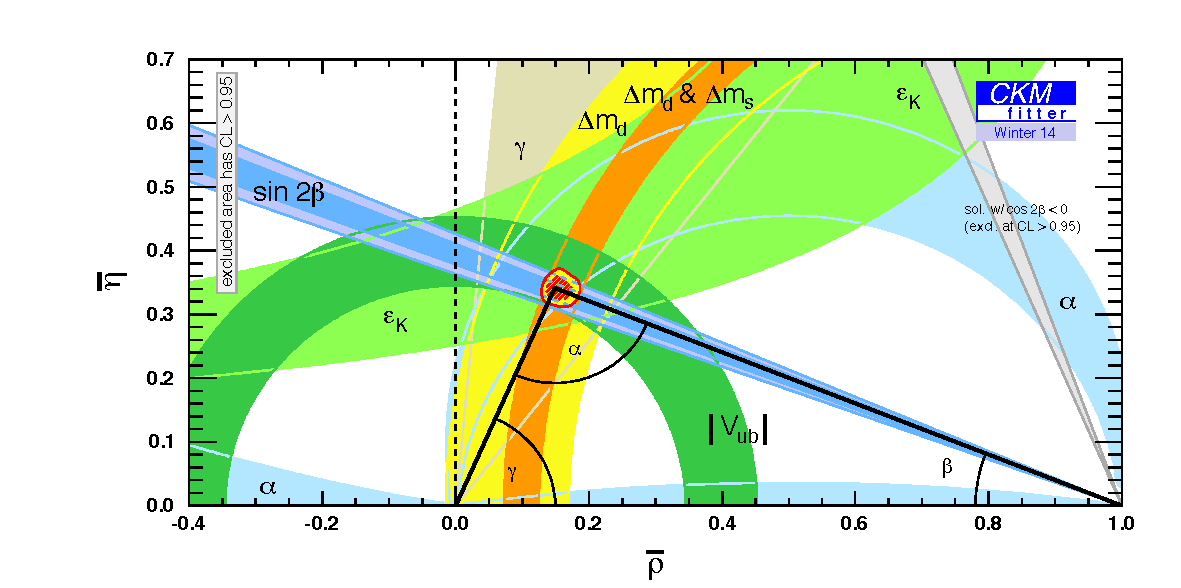
\includegraphics[width=0.65\textwidth]{fig/ckm_fitter.pdf}
	\caption{$C\!K\!M$-Dreieck in der komplexen Ebene. Die farbigen Bänder markieren die Unsicherheiten auf verschiedene Parameter des Dreiecks.\cite{ckm-fitter}}
	\label{fig:ckm}
 	\end{center}
\end{figure}
Bei einer verschwindenden komplexen Phase in der Matrix, also ohne $\CP$-Verletzung, würde die Spitze des Dreiecks auf der reellen Achse liegen, und dieses zu einer Linie entarten.\\ 
In der modernen Teilchenphysik sind diese $C\!K\!M$-Dreiecke von großer Bedeutung. Durch Ausmessen verschiedener Größen der Dreiecke lassen sie sich überbestimmen. Sollten nun experimentelle Daten zeigen, dass ein solches Dreieck nicht schließt, wäre dies ein Hinweis auf Physik jenseits des SM.\\
Im Folgenden soll nun speziell das System der $\Bz$-Mesonen betrachtet werden. Neben der in Abschnitt \ref{sec:mixing} beschriebenen Mischungsasymmetrie lässt sich auch eine $\CP$-Asymmetrie definieren. Dafür wird zunächst die Übergangswahrscheinlichkeit $\left|\left<f\big|T\big|\Bz(t)\right>\right|^2$ berechnet, wobei $\Bz(t)$ ein \B-Meson beschreibt das bei $t=0$ als \Bz erzeugt worden ist ($\Gamma_H\approx\Gamma_L$ für \Bz und \Bzb):
\begin{align}
\left|\left<f\big|T\big|\Bz(t)\right>\right|^2&=\left|\frac{1}{2}\left<f\big|T\big|\Bz\right>g_+-\frac{q}{2p}\left<f\Big|T\Big|\Bzb\right>g_-\right|^2\nonumber\\
&=\frac{1}{4}A_f^2\left|g_+-\frac{q}{p}\frac{\overline{A}_f}{A_f}g_-\right|^2=\frac{1}{4}A_f^2\left|g_+-\lambda_fg_-\right|^2\nonumber\\
&=\frac{1}{4}A_f^2\left(g_+g_+^*+\left|\lambda_f\right|^2g_-g_-^*-\overline{\lambda_f}g_+g_-^*-\lambda_f g_+^*g_-\right)\nonumber\\
&=\frac{1}{2}A_f^2e^{-\Gamma t}\left[\left(1+\left|\lambda_f\right|^2\right)+\left(1-\left|\lambda_f\right|^2\right)\cos\left(\dm t\right)-2\mathcal{Im}\left(\lambda_f\right)\sin\left(\dm t\right)\right]
\end{align}
Analog dazu erhält man
\begin{align}
\left|\left<\overline{f}\Big|T\Big|\Bzb(t)\right>\right|^2&=\frac{1}{2}A_f^2e^{-\Gamma t}\left[\left(1+\left|\lambda_f\right|^2\right)-\left(1-\left|\lambda_f\right|^2\right)\cos\left(\dm t\right)+2\mathcal{Im}\left(\lambda_f\right)\sin\left(\dm t\right)\right]\\
\left|\left<\overline{f}\Big|T\Big|\Bz(t)\right>\right|^2&=\frac{1}{2}A_f^2e^{-\Gamma t}\left[\left(1+\left|\lambda_f\right|^2\right)-\left(1-\left|\lambda_f\right|^2\right)\cos\left(\dm t\right)-2\mathcal{Im}\left(\lambda_f\right)\sin\left(\dm t\right)\right]\\
\left|\left<f\Big|T\Big|\Bzb(t)\right>\right|^2&=\frac{1}{2}A_f^2e^{-\Gamma t}\left[\left(1+\left|\lambda_f\right|^2\right)+\left(1-\left|\lambda_f\right|^2\right)\cos\left(\dm t\right)+2\mathcal{Im}\left(\lambda_f\right)\sin\left(\dm t\right)\right].
\end{align}
Mit diesen Übergangswahrscheinlichkeiten ergibt sich die $\CP$-Asymmetrie zu:
\begin{equation}
A_\CP=\frac{\Gamma\left(\Bzb(t)\rightarrow f_\CP\right)-\Gamma\left(\Bz(t)\rightarrow f_\CP\right)}{\Gamma\left(\Bzb(t)\rightarrow f_\CP\right)+\Gamma\left(\Bz(t)\rightarrow f_\CP\right)}=\frac{2\mathcal{Im}(\lambda_f)}{1+\left|\lambda_f\right|^2}\sin\left(\dm t\right).\label{eq:cpv}
\end{equation}
Dabei ist $\frac{2\mathcal{Im}(\lambda_f)}{1+\left|\lambda_f\right|^2}$ die $\CP$-verletztende Größe, die hier mit $S_\CP$ bezeichnet werden soll und aus dem in Abbildung \ref{fig:ckm} gezeigten Dreieck den Winkel $\beta$ enthält: 
\begin{equation}
A_\CP=S_\CP\sin\left(\dm t\right)=\sin\left(2\beta\right)\sin\left(\dm t\right)
\end{equation}

